\xchapter{Our variability based model for Public Communication of Emergencies}{}\label{sec:variabilityModel}

Based on the results of our research of the good practices for public communication of emergencies, in the results obtained in the two workshops carried out with specialists in public communication and our analysis of variability in the whole process of public communication, we propose a variability based model that provides a complete support in the task of public communication of emergencies.   

\begin{figure}[ht!]
\begin{center}
  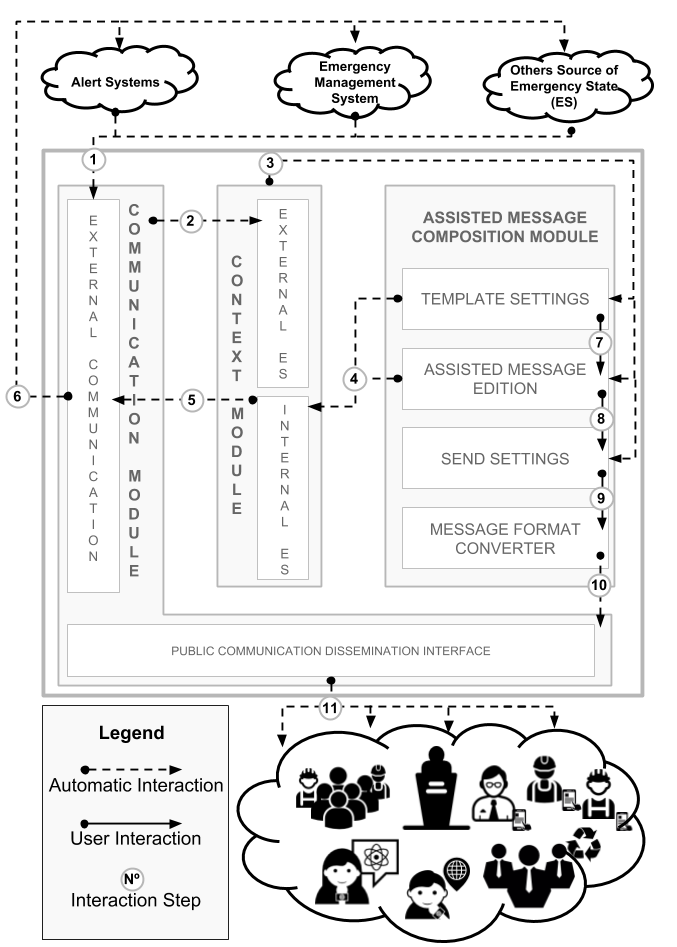
\includegraphics[width=\linewidth, keepaspectratio]{images/ConceptualModel.png}
\caption{Our Variability Based Model to generate and disseminate Emergency Public Communications}
\label{fig:ConceptualModel}
\end{center}
\end{figure}

Figure \ref{fig:ConceptualModel} presents our proposal of a variability based model to generate and disseminate Emergency Public Communications. We will present our model according to the Steps of Emergencies directly linked to the tasks of creation and dissemination of public communications: Verify the Situation, Prepare Information and Release Information through Prearranged Channels.

\section{Verify the Situation}

The task of communicating the public about the occurrence of an emergency and its consequences begins with the search of reliable information. Situational awareness is essential to guarantee that only consistent information will be transmitted to the public and thereby achieve gain the public's confidence. 

In some cases, the reliable information can be obtained in other software of emergency management or alert systems. Because of this, the first interaction described in our model is an automatic search of information in external systems. The responsibility of the communication module, more specifically, the sub-module of External Communication is to implemented interfaces that periodically and automatically get information from external sources and provide it to the context module (interaction 2). 

The set of information obtained from external source composes the External Knowledge in the Context Module. We call from Internal Knowledge the information obtained by the input of the users during the interaction within the Assisted Message Composition Module (AMC) (Interaction 4). The Context Module is responsible for automatically management the information of the Internal and External Knowledge and to provide the most recent information to the AMC module (Interaction 3).

Commonly, some information about the emergency is not obtained from External Source of information. This information probably will be included during the composition of emergency public communication by the emergency communication team. In this case, it is important to share this information for the others Emergency Management Systems. Because of this, the Internal Knowledge is automatically sent to the External Communication Sub-module (interaction 5) which, in sequence, share this information with external systems (interaction 6).


\section{Prepare Information}

The process of creation of public communications begins with the configuration of the Template Message. Some characteristics are essential to define the appropriate template for the current emergency. We generate the most appropriated model according to the response of 4 questions: \textbf{WHAT happened?} (what is the type of emergency); \textbf{WHAT is the current status?} (what is the current phase of emergency); and \textbf{WHICH and HOW the target audience will be communicated?} Some of these questions are linked to the emergency state. So, the Template Settings sub-module can consume (interaction 3) or provide (interaction 7) information to the Context Module. 

The main contribution of our work is the semi-automated approach to building public communications. We map the variability in the composition of public communications messages and as a result, we create structured templates that adapt to the current emergency state in order to reduce the necessity of interactions to compose the public communication.

After obtaining the essential information about the communication of emergency, the Assisted Message Edition sub-module generate a dynamic template according to these information (interaction 7). This process includes the exclusion of sentences exclusive for specifics target audiences (that are not targets of this communication) or emergency type (different of present emergency). %Figure \ref{fig:step2} present our conceptual propose of an user interface to configure the public communication model in order to generate multiples public communications.

In addition, it is necessary to configure the sentences according to the present emergency status. We observed a relationship between emergency characteristics and the content of public communications in the variability of content according to the status of emergency. There are four generic types of variation in the content of a sentence depending on the state of the emergency, the variation can be either: 

\begin{enumerate}
   \item A direct association, where the value of the variable information is an emergency state data;
   \item An indirect association, in which the value of the variable information depends on an emergency state data, but it does not have the same value;
   \item Based on the occurrence (or not) of a fact, which might come from the emergency state; or
   \item An information not associated with the emergency state.
\end{enumerate}

Figure \ref{fig:sentenceContext} shows practical examples of each different behaviour identified and its influence on the content of the sentences.

\begin{figure}
\centering
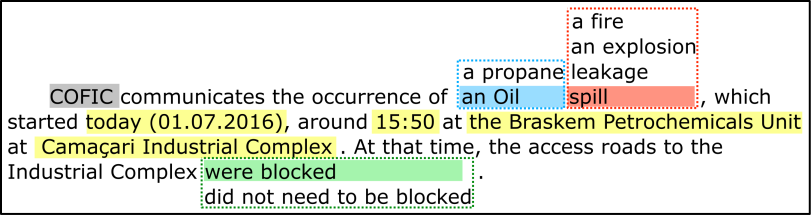
\includegraphics[width=0.75\linewidth]{images/sentenceContext.png}
\caption{Examples of different behaviour on the content of sentences according to the emergency status}
\label{fig:sentenceContext}
\end{figure}

The information marked in yellow, in the example, are the content that has a direct association with the emergency state, like emergency start date and time, the name of the affected company and so on. This information was put directly into the content of the sentence.

In red, we present an example of indirect association between emergency state and part of the sentence. The sentence will read ``a fire'' in case the emergency type is ``FIRE'', ``an explosion'' in case the emergency type is ``EXPLOSION'', ``leakage'' in case of ``GAS LEAKAGE'' emergency, and ``spill'' in case the emergency type is ``ENVIRONMENTAL''. 

We used green to represent a sentence in which the variable content is based on the occurrence or not of a fact. In this case, the occurrence or not of road blocks. 

An example of sentence not associated with the emergency state is given in grey. The name of the company that is responsible for handling the crisis, in this case, is an information about the system configuration (e.g. the company that the emergency public communication team is associated).

Finally, an example of qualifier for the emergency type is shown in blue. The leaked material is a type of information associated with the incident ``GAS LEAKAGE'' or ``ENVIRONMENTAL''.

\section{Release Information through Prearranged Channels}

Disseminate the public communication through the most appropriate communication channel for each target audience is essential to help ensure the success in the public communication of an emergency.

In the Send Setting sub-module, the user can select the dissemination area, email and cell-phone list and other configurations of the selected communication channels. After that (interaction 9) the Message Format Converter (MFC) sub-module generate the specific message for each target audience from the Structured Template ( a result of the Assisted Message Edition sub-module).  After that, the MFC needs to convert each message to the appropriated format to be send by each communication channel (interaction 10). 

Finally, the messages are sent automatically by the Public Communication Dissemination Interface (interaction 11). It is in this Interface that is implemented the logic to send messages for each communication channel. 

We propose an interface that has been projected to enable a fast configuration of target audience. The main idea is automatise, when possible, the selection of information about the target audience selected previously. To do so, we group different send setting by pre-defined areas. For example, in a pre-defined area, like a neighbourhood community of an industrial park, we can associate automatically a phone number list of residents to send SMS or use the coordinates to send geo-referenced messages by a Mobile App.

